\section{Implementation}
Simulation, as well as visualization, was implemented in python using object oriented programming paradigm, all elements are kept in a single repository on GitHub\cite{repository}. It was crucial for the project to separate those entities to ensure seamless testing possibilities as well as recreating animation from previously performed simulations. For testing purposes simulation can also be run using multi-threading, taking input from standard input, in particular test files with specified parameters of the simulations. It makes plotting and testing faster as simulations with many cars can be time-intensive.

\subsection{Simulation}
Simulation is a part of the project which produces specific output from given parameters, imitating real-world behavior. All classes implemented can be seen on a diagram in appendix \ref{appendix:classDiagram}. The main class responsible for performing the simulation is a Scheduler class. It is taking several parameters as an input which can be seen below:

\begin{itemize}
    \item Average driver mood
    \item Number of lanes
    \item Entry lane attributes
    \item Highway length [km]
    \item Speed limit [km/h]
    \item Proportion of Autonomous cars
    \item Proportion of Trucks
\end{itemize}

An instance of this class is storing the mentioned parameters as constants for the simulation and propagating them to all subordinate classes. All parameters given are being translated to SI units before propagation. In the initial architecture, it was decided to make a fixed time step in the simulation, equal to one second.

When initialized, the scheduler creates an instance of the Highway class with a given number of Lanes instances, speed limit, length, and other properties. This object will later be used to render the simulation.

There are two options to perform simulations, either manual or automatic. The former can be used to create a specific simulation with full control over the state and object. It requires manually calling the step function which is updating the simulation. The advantage of this option is that all parameters can be changed in between the steps but it also requires a lot of manual labor and steps.

The automatic simulation takes two arguments to be able to perform actions: Inflow [vehicle/minute], Simulation time [s]. After being called, it is performing several steps equal to the simulation time. In between steps, the scheduler is deciding if and where to spawn the vehicles to achieve set inflow on a highway. Every action involved in a simulation and a step function can be seen in figure \ref{fig:sim-steps}.

\begin{figure}[H]
    \centering
    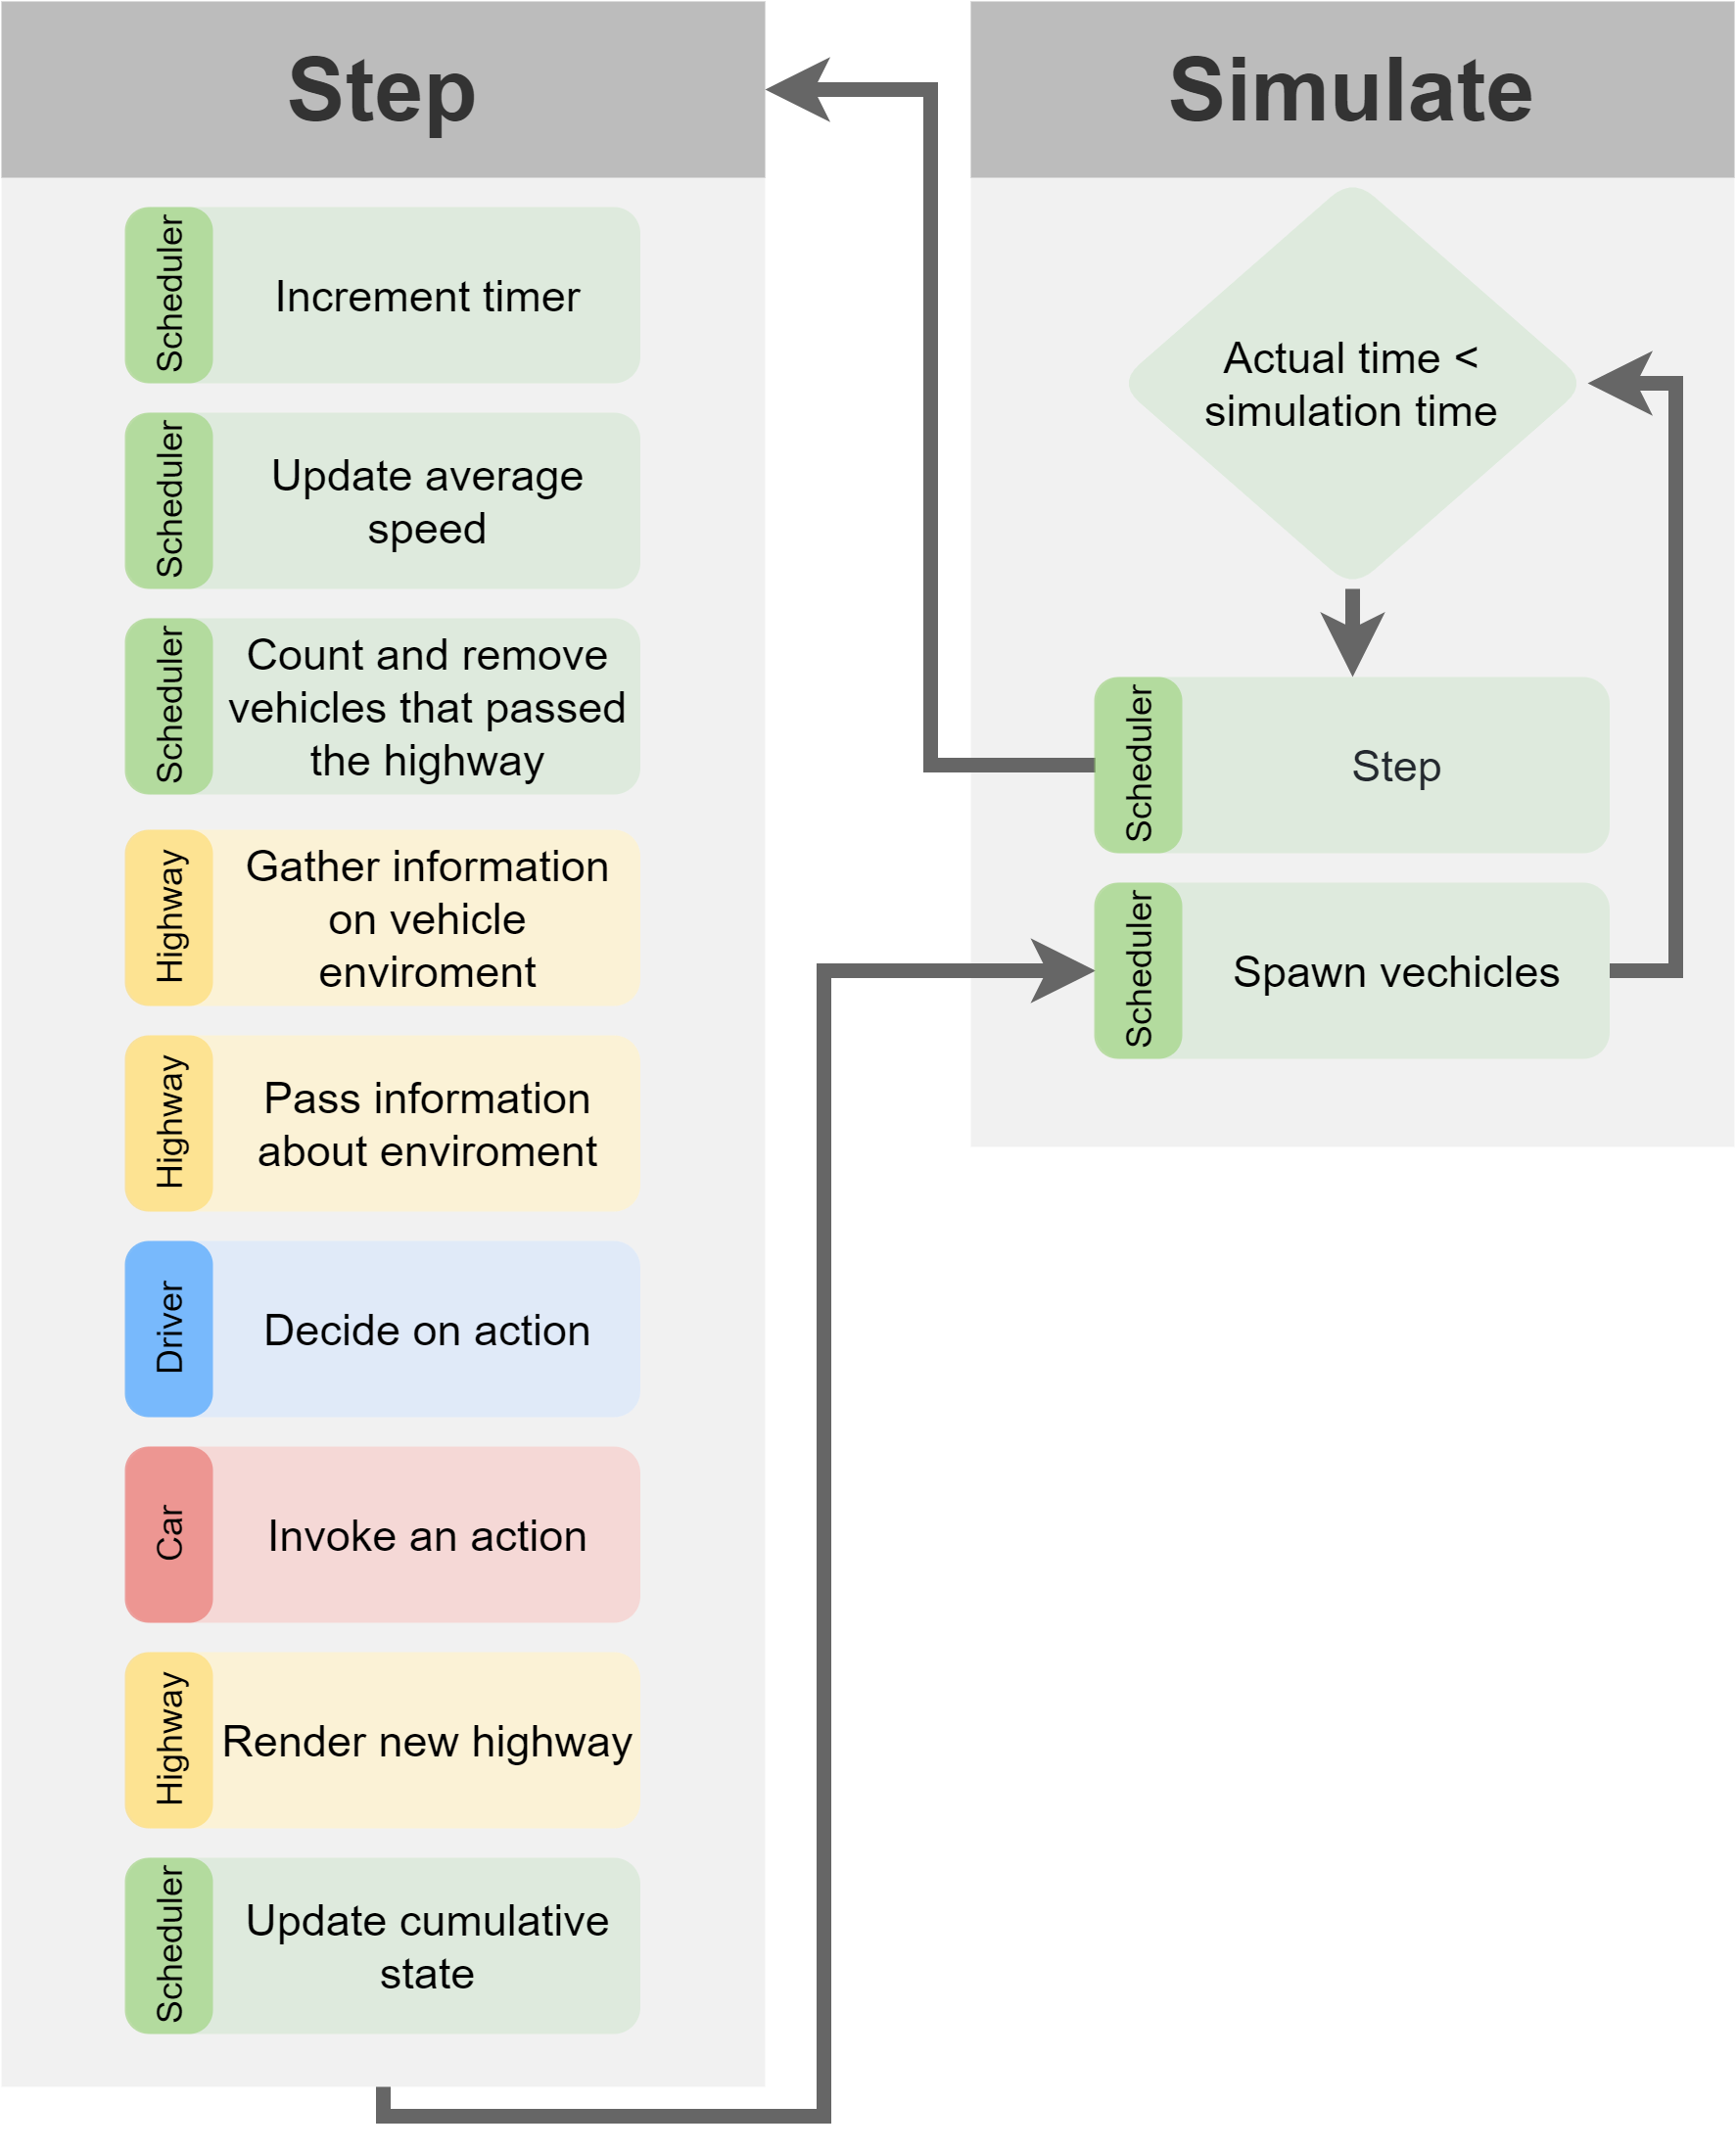
\includegraphics[width= \linewidth]{images/simulation-steps.png}
    \caption{Logic behind simulation.}
    \label{fig:sim-steps}
\end{figure}

To generate the vehicles, the scheduler is choosing between spawning different types of vehicles( Car, Truck or Autonomous car) with the probabilities given as a desired proportion of the vehicles on a final Highway object where:

\begin{multline}
    \begin{gathered}
        {P(autonomous\ car)}=proportion\ of\ autonomous\\
        {P(truck)}=proportion\ of\ truck\\
        {P(car)}=1-proportion\ of\ truck\ - proportion\ of\ truck
    \end{gathered}
\end{multline}

For Car and Autonomous car, the speed of the vehicle is being chosen from a normal distribution in relation to the speed limit on a highway:

\begin{multline}
  vehicle\ speed = \mathcal{N}(speed\ limit,\,(0.1*speed\ limit)^{2})
\end{multline}

To make the simulation easily extensible by adding new types of vehicles polymorphism and inheritance were introduced. Any type of vehicle can inherit from the Car class and change the behavior by setting different parameters and overloading take action method(figure \ref{fig:polymorphism}), f.e Autonomous car is taking an action not only based on the driver's decision but also it's own knowledge about the environment. For now, there are three vehicles types implemented: Truck - slow, and not willing to take many actions, Autonomous car - an entity that considers the position and speed of the other autonomous cars to decide on an action, Car - normal car vehicle, controlled by a driver. Every vehicle includes a Driver class instance as a parameter and invokes an action based on its decisions and in some cases additional knowledge(Autonomous car).

\begin{figure}[H]
    \centering
    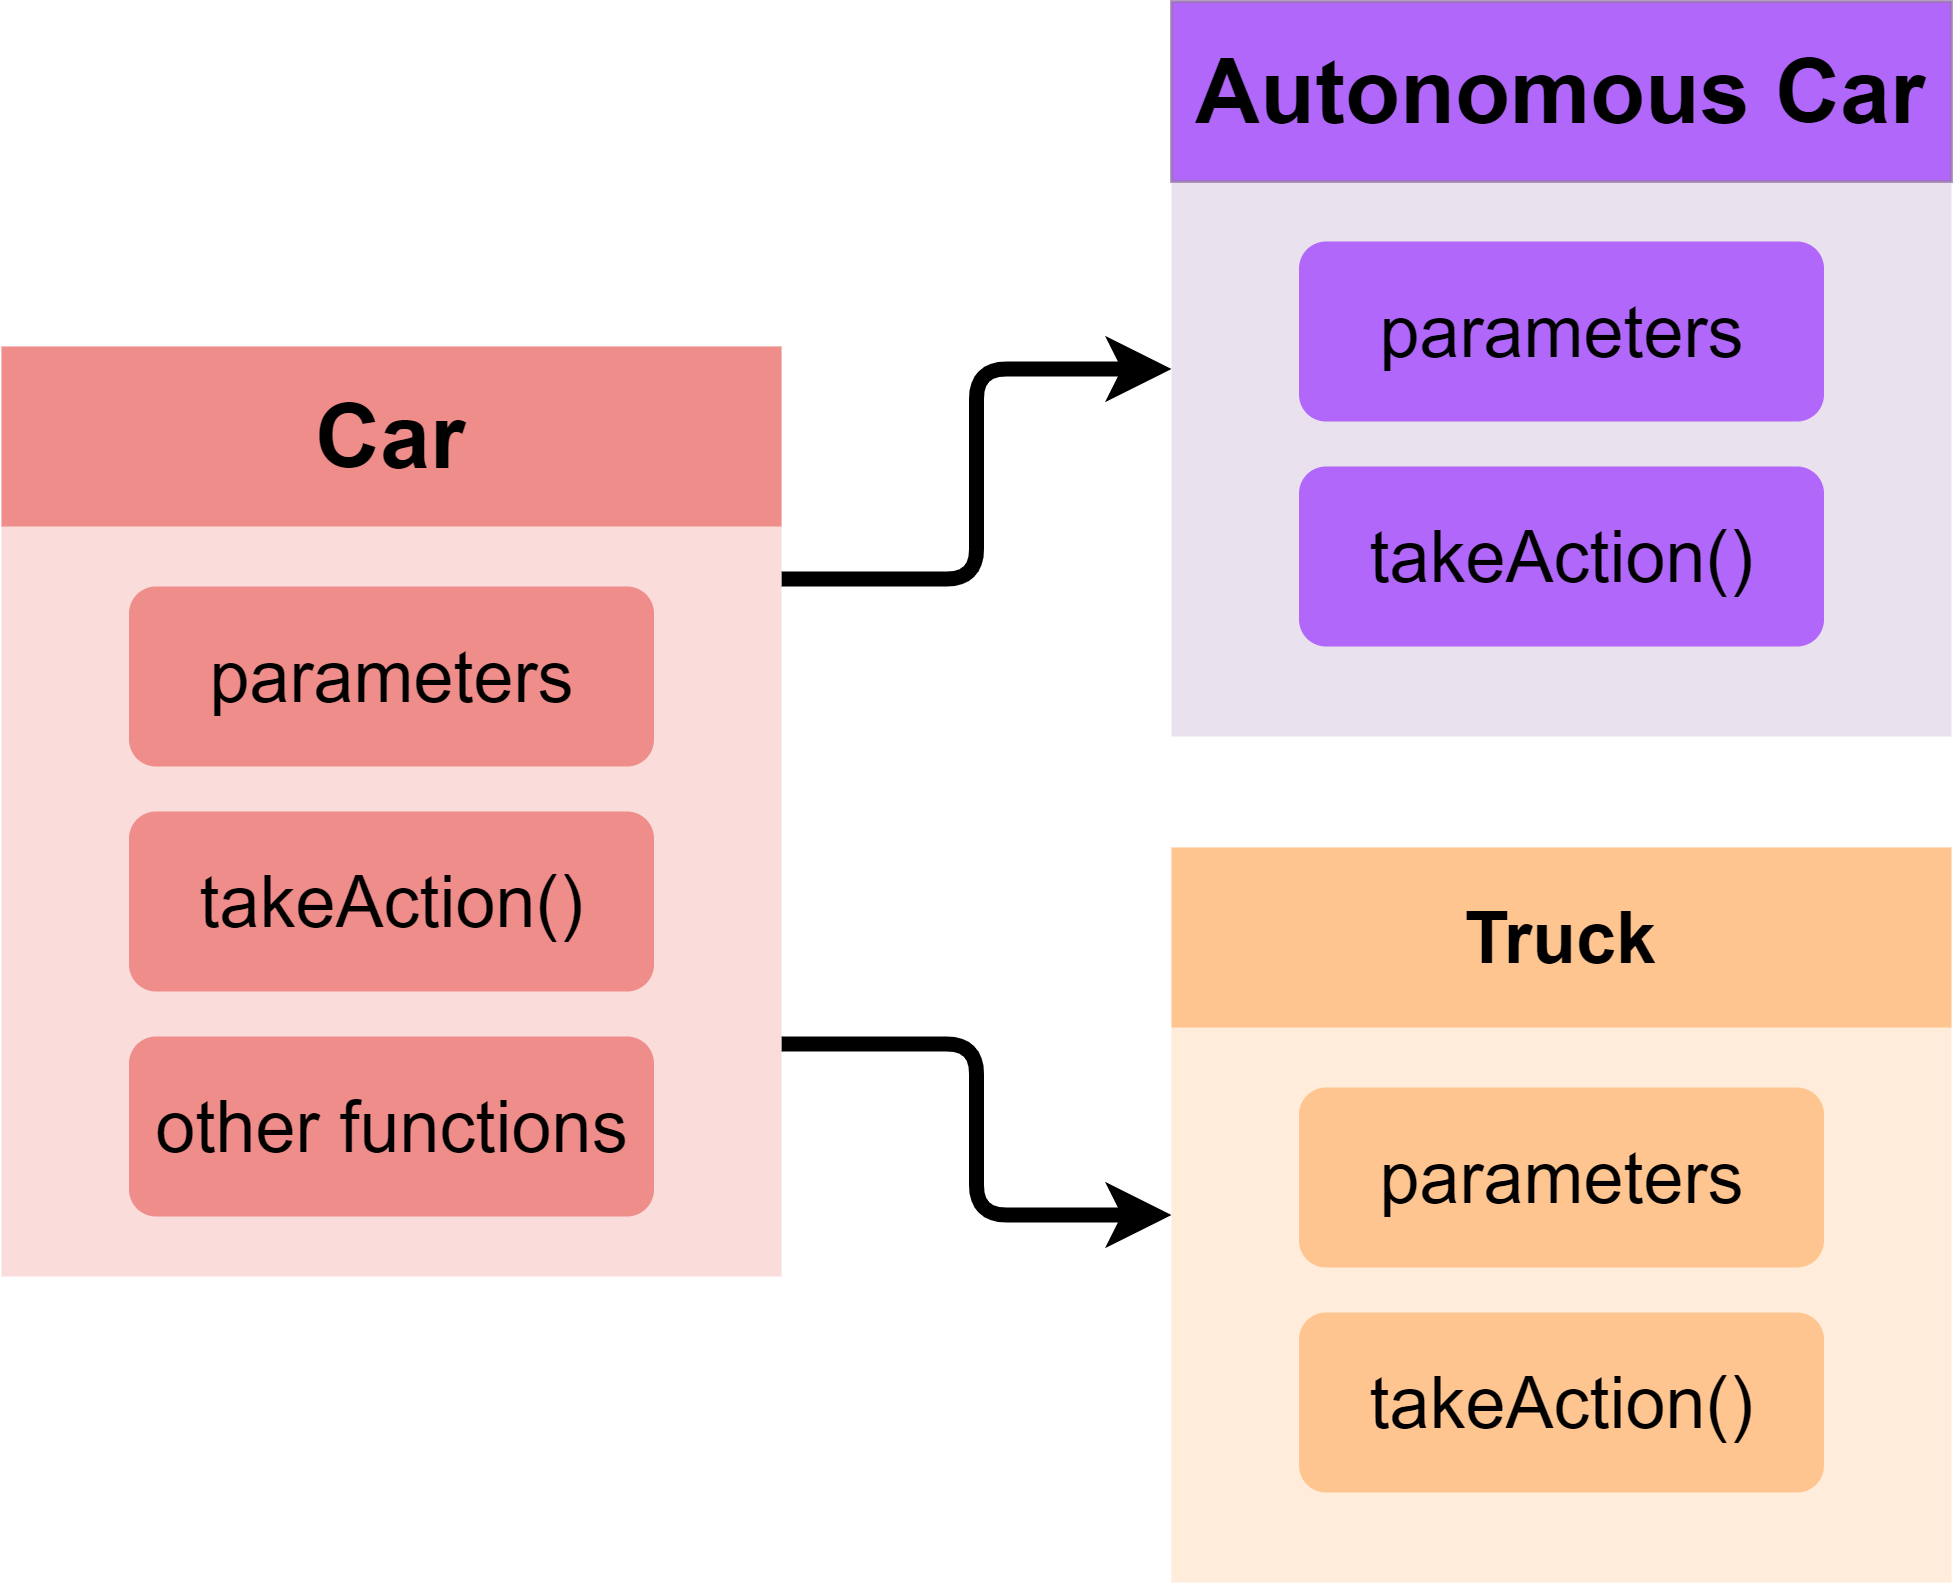
\includegraphics[width=0.9\linewidth]{images/polymorphism.png}
    \caption{Logic of polymorphism.}
    \label{fig:polymorphism}
\end{figure}

Additional capabilities of the simulation:
\begin{itemize}
    \item Exporting state to JSON file.
    \item Exporting the whole scheduler to a pickle file.
    \item Importing both state and scheduler from the file.
    \item Resetting scheduler state to build a new simulation with the same parameters.
\end{itemize}

\subsection{Visualization}
It was decided to make a simple visualization based on pythons matplotlib library\cite{Hunter:2007}, more specifically its animation function. As visualization is completely separated from simulation it can directly take the dictionary generated by simulation or fetch the input from a valid JSON file. Validity means that it has to follow a certain structure(as generated from the scheduler class), presented in the appendix \ref{appendix:json-schema}.

The visualization module is then plotting each step of the simulation as one frame of the final animation, where the x-axis represents the distance from the beginning of the highway and the y-axis represents the lane. Cars are being colored in relation to their unique id, there is also an option to color them based on the class of the vehicle which can be seen in appendix \ref{appendix:color-output}. The outcome can be presented interactively as a matplotlib plot or exported to a GIF file, the latter usually works better as it is more smooth. Representation of a single highway with 5 lanes can be seen in figure \ref{fig:single-highway}, color coding is based on the unique id of a car.

\begin{figure}[H]
    \centering
    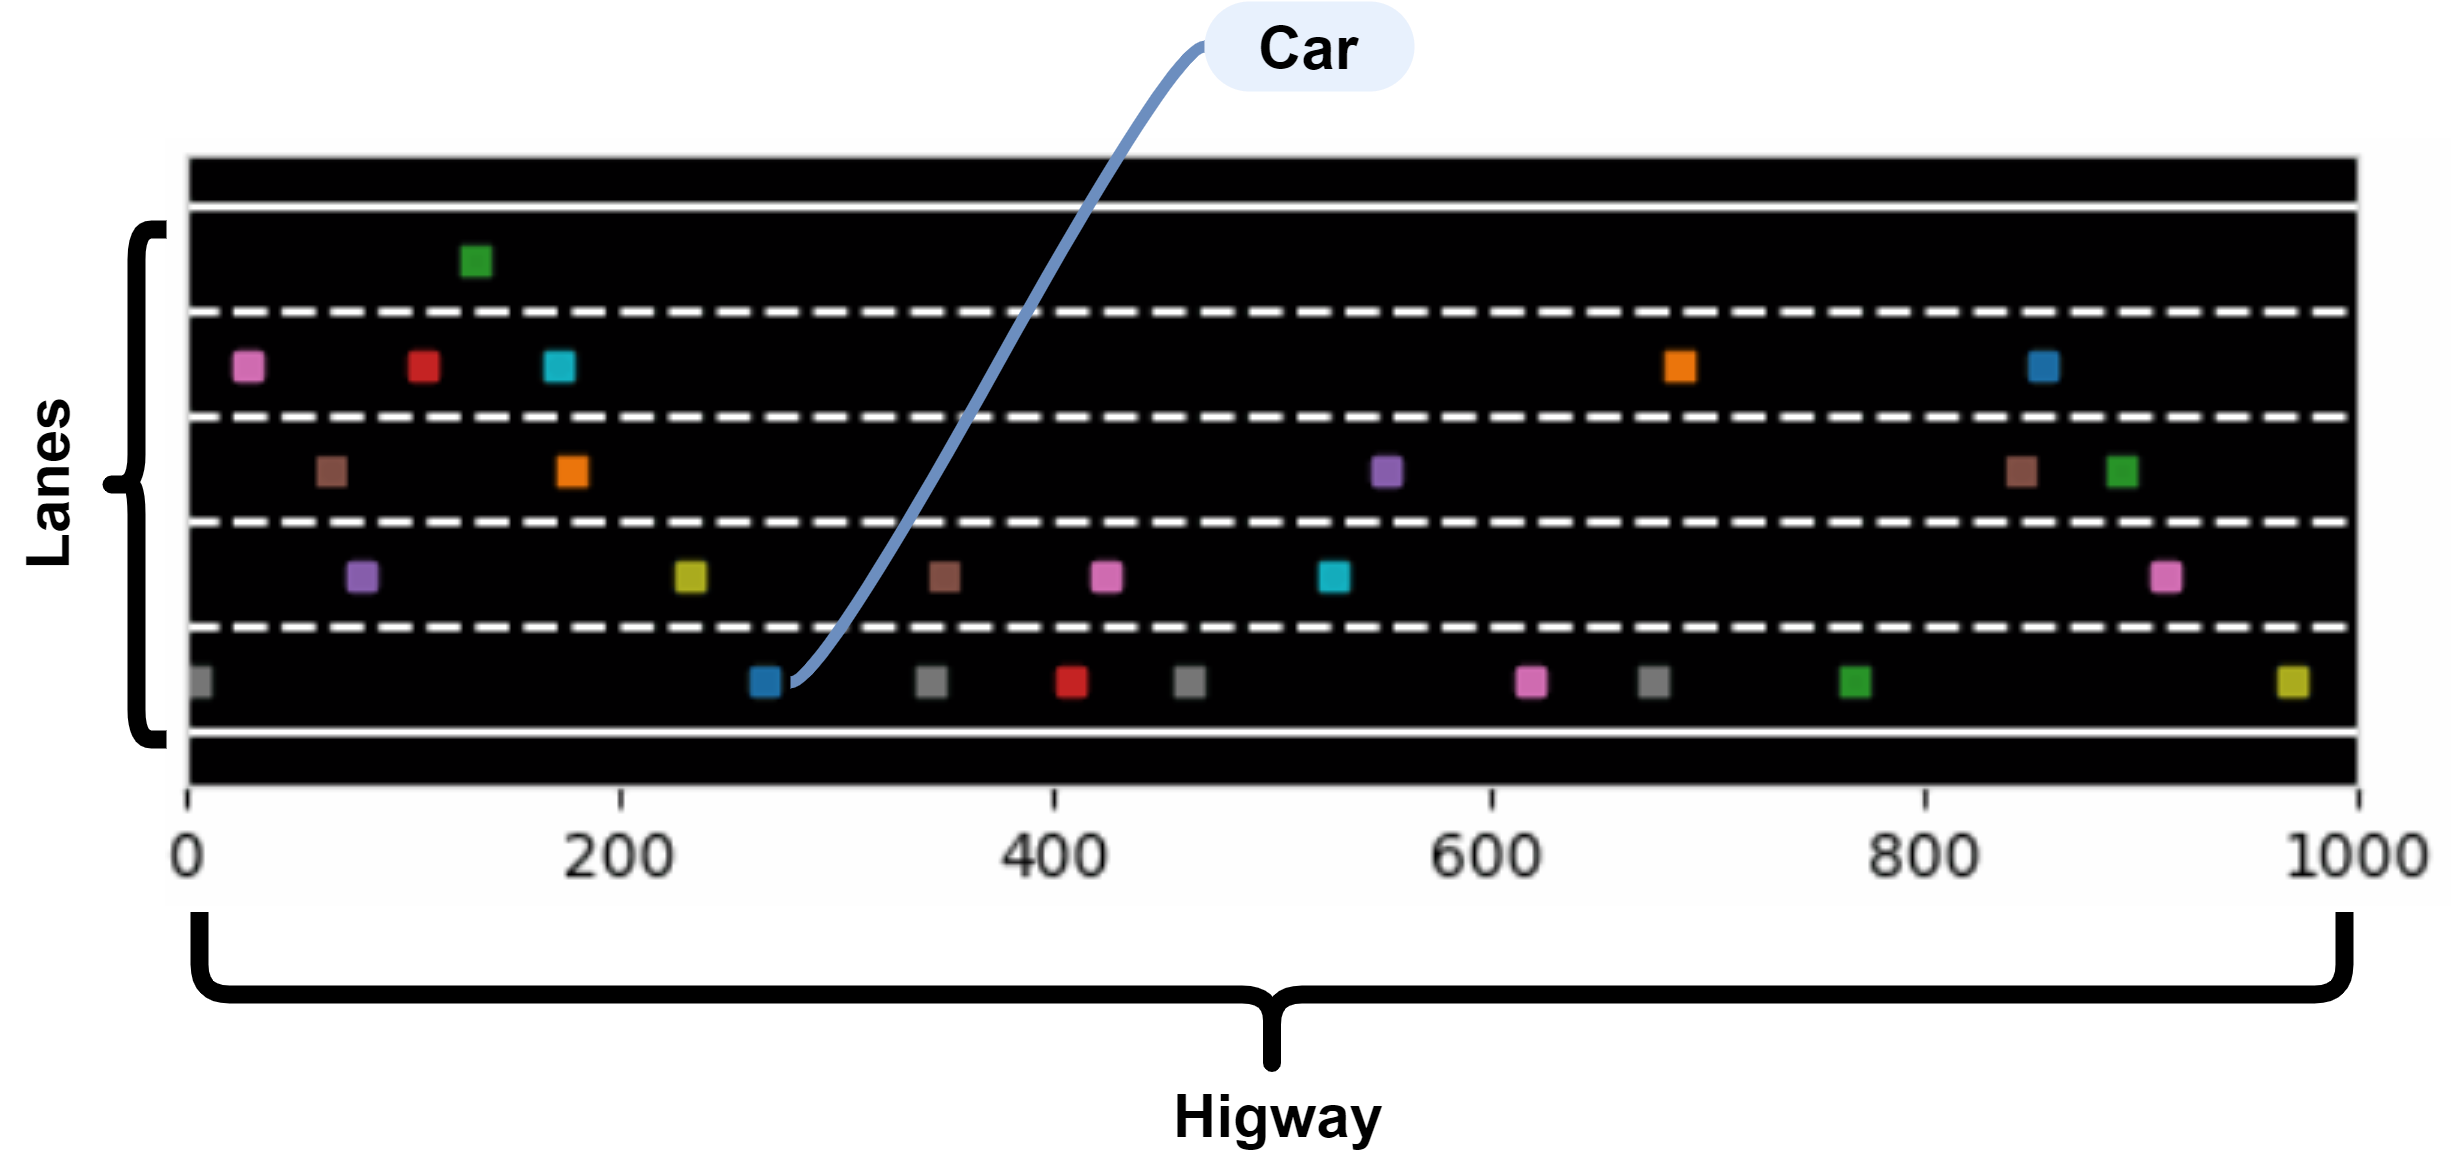
\includegraphics[width=\linewidth]{images/single-highwa.png}
    \caption{Single highway animation.}
    \label{fig:single-highway}
\end{figure}

Visualization can be made from multiple simulations with different parameters, and it is automatically adjusting all plots, additionally, the speed of the simulation can be adjusted by tweaking two parameters: data reduction and animation speed. Results from the simulation can be seen in real-time in form of a bar plot that indicates current vehicle flow on the highway and a line plot that shows average speed on each simulation. 

Complete animation outcome can be seen on figure \ref{fig:animtion}.
\begin{figure}[H]
    \centering
    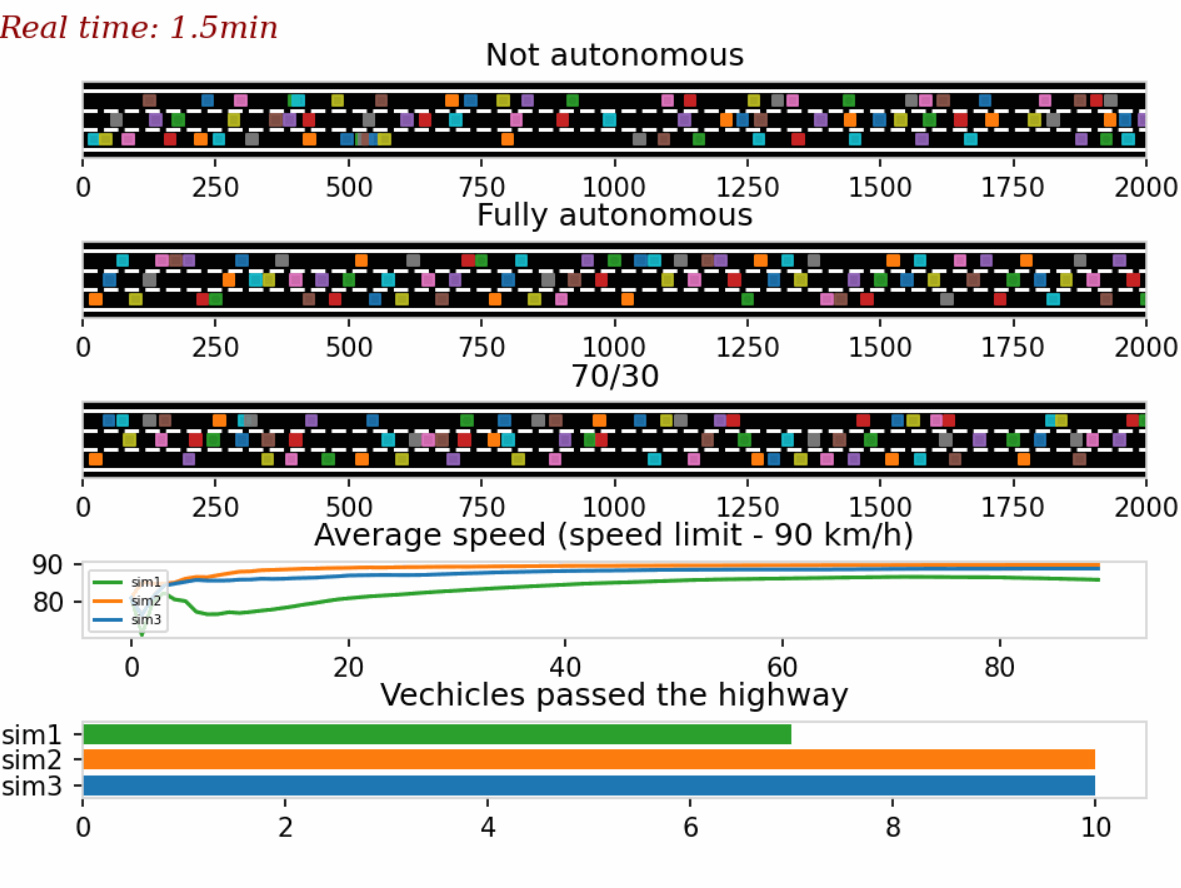
\includegraphics[width=\linewidth]{images/sim-1.png}
    \caption{Example of animation with 3 different simulations.}
    \label{fig:animtion}
\end{figure}

More detailed animation outcomes with color-coding based on a type of vehicle can be found in appendix \ref{appendix:color-output}.